%!TEX root = ../thesis.tex
%%--------------------------------------------------------------------------
%% ADOCK
%%--------------------------------------------------------------------------

%% REMEMBER:
%% - section
% \section{Section Title}
% \label{sec:section_title}
%
% - subsection
% \subsection{Subsection Title}
% \label{sub:sub_title}
%
% - paragraph
% \subparagraph{Paragraph Title}
% \label{subp:subp_title}


% --------------------------------------------------------------------------- %
% ---------------------------------- ADOCK ---------------------------------- %
% --------------------------------------------------------------------------- %


\section{Our Solution, aDock}
\label{sec:adock_intro}
The lack of a uniform and standardized test environment for cloud systems brought us to develop aDock.\\
aDock is a suite of tools that lets the final user deploy a complete OpenStack system; run simulations against it; collect output data and view results on a friendly user interface.\\
We chose OpenStack as cloud computing software platform, because of its open-source nature and because of its continuous evolution with the aim of keeping up with the last cloud standards.\\
Our intended users are OpenStack developers who need to run their code in a fully functional environment and researchers who want to try their algorithm on a complete cloud system to test out its behavior.

\section{Requirements}
\label{sec:adock_reqs}
In this section, we will identify both functional and non-functional requirements for aDock.

\subsection{Functional Requirements}
\label{sub:func_req}

\paragraph{FR1}\label{p:fr1} \emph{aDock should provide tools to deploy a complete environment.} \hfill \\
A user should be able to start and update OpenStack's nodes with a single command. aDock should provide the user with an abstraction of a server called ``node''. The ``node'', in its depth, is an Ubuntu based Docker container, shipped with OpenStack services dependencies. A user should be able to decide which services will be installed and started on each node and their internal configuration using a configuration file.
\subparagraph{Solution} FakeStack (see section \ref{sec:fakestack}) is the aDock module which provides the user with the specified tools. Starting a node is as easy as \code{\$ run\_node}. A node can be configured by means of a simple configuration file. Nodes are of two types, \textit{controllers} and \textit{computes}. Controller nodes are different from compute ones because they are shipped with \textit{MySQL} and \textit{RabbitMQ} installations.

\paragraph{FR2}\label{p:fr2} \emph{aDock should provide a tool to run simulations.} \hfill \\
If the user puts his/her code into OpenStack he/she probably aims at running simulations and examine the new piece of code behavior in interacting with the entire system. Simulations should be configurable according to the user needs and repeatable.
\subparagraph{Solution} Oscard (see section \ref{sec:oscard}) is the aDock module which takes care of running repeatable and configurable simulations against an OpenStack system.

\paragraph{FR3}\label{p:fr3} \emph{aDock should persistently store simulations output.} \hfill \\
Once a simulation has been run, it could be interesting to store the outputs of it in terms of generic metrics about the system, such as the average of the number of compute nodes active during the simulation, the average of virtual CPUs used and so on.
\subparagraph{Solution} Oscard, by default, stores the aggregates of a simulation into a Firebase\footnote{\url{https://www.firebase.com/}} backend. In our case, the backend is called Bifrost (see section \ref{sec:others}).

\paragraph{FR4}\label{p:fr4} \emph{aDock should provide a user interface} \hfill \\
Although Firebase provides an interactive user interface, data is displayed in a \textit{JSON} fashion and it is, therefore, not easily understandable and browseable. Simulations results should be displayed to user in a friendly manner, using charts to give the user a glimpse of the current situation. Data representation should be given in real-time.
\subparagraph{Solution} Polyphemus (see section \ref{sec:others}) is the aDock module which takes care of displaying to the user real-time simulation results in a friendly manner.

\paragraph{}\label{p:adock_archi} aDock turns out to be a modular system where each component is configurable and has a precise purpose. FakeStack is employed to start nodes; Oscard runs simulations and collects aggregates on Bifrost; Polyphemus is the eye on the data that shows the user the results obtained.
In figure~\ref{fig:adock_high_arch} we highlight the general architecture of aDock.

\todo{make aDock high-level architecture!}

\subsection{Non-Functional Requirements}
\label{sub:nonfunc_req}
As opposed to functional requirements, aDock has very strong non-functional requirements in order to give a suitable testing environment to our stakeholders. In general we take leverage of Docker and DevStack and use their biggest strength. Docker gives us high speed in running containers and sandboxing by construction and makes aDock cross-platform; while DevStack gives us great flexibility and configurability for what concerns OpenStack services.

\paragraph{NFR1}\label{p:nfr1} \emph{Users should be able to choose which code is running in OpenStack.} \hfill \\
Before booting the entire system the user should be able to choose if he/she wants to run OpenStack code from a precise code repository which is, in general, the better and more supported way to version and share code among developers and even physical machines. Speaking in Git\footnote{\url{http://git-scm.com/}} terms, a user could choose to run the most up to date code (which may be buggy) and so get the code from branch \code{master}, or maybe get a much more stable OpenStack version and get the code from branch \code{stable/juno}. The most interesting fact (and this is the scenario we have in our mind) is that the user could choose to fork an OpenStack service and see his/her code running onto nodes.

\subparagraph{Solution} All of this is achievable thanks to DevStack, which installs OpenStack services cloning repositories from GitHub and running \code{python setup.py install}. By default, DevStack clones official OpenStack repositories from branch \code{master}, but it is possible to specify different repository URLs and branches for each of the OpenStack services by means of \code{local.conf} files.

\paragraph{NFR2}\label{p:nfr2} \emph{aDock should be lightweight.} \hfill \\
Users often need to test algorithms that, by design, target the management and/or optimization of tens of physical servers. Since we can assume that not everyone will have that amount of resources, we believe that aDock should be as light-weight as possible. It should be possible to run aDock on limited hardware, potentially even on one's personal laptop. It is under this assumption that sandboxing becomes important; indeed, the experimentation environment should not have any sort of repercussions on the user's machine; we want the user to be able to build and tear down the environment with no consequences.

\subparagraph{Solution} Docker is a virtualization system which relies on Docker containers which are much more lightweight than virtual machines\footnote{\url{http://devops.com/blogs/devops-toolbox/docker-vs-vms/}} \todo{is the ref authoritative?}. Docker gives us, by construction, speed and lightness.

\paragraph{NFR3}\label{p:nfr3} \emph{The experimentation environment should be highly configurable.} \hfill \\
Our primary goal with aDock is to provide a fast and easy way to create the experimentation environment. We believe that building a system which allows users to design the overall architecture of the cloud system is out of scope of this thesis, mainly because of the intrinsic high complexity and vastness of OpenStack's system itself. Up to now, as a proof of concept, we will focus on ``1 + N'' architecture, with $1$ controller node and $N$ compute nodes.

\subparagraph{Solution} The possibility to configure the system still remains in configuring OpenStack services in terms of their internal behavior. This is achieved, again, thanks to DevStack, which allows us to configure OpenStack in all its aspects through \code{local.conf} file. Each service can be configured in each of DevStack installation phases. Each service, during installation, passes through \textbf{local}, \textbf{pre-install}, \textbf{install}, \textbf{post-config}, \textbf{extra} phases\footnote{\url{http://docs.openstack.org/developer/devstack/configuration.html\#local-conf}}. Configuring a service is as simple as adding few lines to \code{local.conf} file:

\begin{lstlisting}[title=Adding per-service configuration to DevStack's local.conf file]
... # DevStack configurations

[[post-config|\$NOVA-CONF]]
[DEFAULT]
verbose=True
logdir=/var/log/my-nova-logdir

# SCHEDULER
compute_scheduler_driver=nova.scheduler.MyMagicScheduler
# VIRT DRIVER
compute_driver=nova.virt.fake.MyAmazingFakeDriver
\end{lstlisting}


\paragraph{NFR4}\label{p:nfr4} \emph{aDock should allow users to run repeatable simulations.} \hfill \\
It is of paramount importance that users be able to compare their results with baseline approaches, as well as with related work from the state of the art. aDock should make it easy to compare an experiment's results with those of others on the same simulations.

\subparagraph{Solution} Oscard will take into account repeatability both giving the possibility to run the same simulation, at the same time, on multiple hosts, both using pseudo-randomization (see section \ref{sec:oscard}).

% --------------------------------------------------------------------------- %
% -------------------------------- FAKESTACK -------------------------------- %
% --------------------------------------------------------------------------- %

\section{FakeStack}
\label{sec:fakestack}
FakeStack is the aDock module which allows the user to manage \textit{nodes}, which are the building blocks of an OpenStack system. Nodes are of two types: \textit{controllers} and \textit{computes}. Both of them are Ubuntu-based Docker containers shipped with pre-installed software that satisfies most\footnote{main services as \textit{Nova}, \textit{Keystone}, \textit{Glance} are actually supported.} of OpenStack's services dependencies. Both controller and compute nodes are configurable by means of simple configuration files ~\ref{sub:fakestack_conf}.\\
FakeStack provides a set of scripts to handle node startup, service updating on live nodes and other features~\ref{sub:fakestack_scripts}.

\subsection{Nodes}
\label{sub:fakestack_scripts}
As already anticipated in requirement~\ref{p:nfr3}, we will focus on ``1 + N'' architectures. This architecture is characterized by $1$ controller node that handles $N$ compute nodes.\\
The main difference between a controller and a compute node is the presence, in the first one, of database (in our case, \textit{MySQL}) and message broker (in our case, \textit{RabbitMQ}) services, compulsory for OpenStack's controller nodes.

To understand how FakeStack really works, it is useful to examine its internal structure:

\begin{figure}[!ht]
\centering{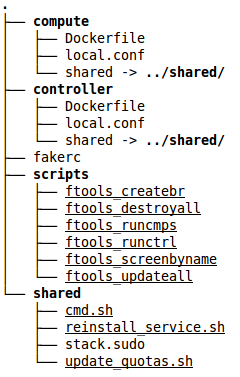
\includegraphics{images/fakestack_tree.png}}
\label{fig:fakestack_tree}
\caption{FakeStack's file structure}
\end{figure}

As we can see in figure~\ref{fig:fakestack_tree}, nodes have two separated \texttt{Dockerfile}s (which makes them two different Docker containers), but they share a set of scripts contained in \texttt{shared} folder:

\begin{description}
	\item[cmd.sh] This is the script that will be run when the container starts (\code{docker run}). In algorithm~\ref{alg:cmd.sh} we explain its behavior in terms of pseudo-code.
	\begin{algorithm}[H]
	\caption{\texttt{cmd.sh} behavior}
	\label{alg:cmd.sh}
	% 1 is for "number any line", 0 for "no"
	\begin{algorithmic}[0]
		\If{node is \emph{controller}}
			\State set last IP in Docker bridge \Comment{assign static IP address to \emph{controller}}
		\EndIf

		\State ping 8.8.8.8 \Comment{Check internet connection}

		\If{node is \emph{controller}}
			\State start \texttt{mysql}
			\State start \texttt{rabbitmq-server}
		\EndIf

		\State \textbf{./stack.sh} \Comment{real OpenStack installation (using DevStack)}

		\State /bin/bash \Comment{let the user work on the container}
	\end{algorithmic}
	\end{algorithm}
	

	\item[reinstall\_service.sh]
	\item[update\_quotas.sh]
\end{description}

Once a node has been built, all of this shared scripts are copied to the file-system of the node.\\
\texttt{local.conf} file, instead, is bound\footnote{\texttt{local.conf} is a \href{https://docs.docker.com/userguide/dockervolumes/\#data-volumes}{\textit{Data Volume}}. Basically it is a file whose modifications are visible at each container's run.} to node's file-system avoiding rebuilding at each modification.

When a node is started, \texttt{cmd.sh} will run, resulting in running DevStack's \texttt{stack.sh}. It is at this moment that OpenStack's installation starts~\ref{} \todo{reference to DevStack's detailed description}.

\subsection{Scripts}
\label{sub:fakestack_scripts}

\subsection{Configuration}
\label{sub:fakestack_conf}
using DevStack's syntax ...

\subsection{Example}
\label{sub:fakestack_ex}

% --------------------------------------------------------------------------- %
% ---------------------------------- OSCARD --------------------------------- %
% --------------------------------------------------------------------------- %

\section{Oscard}
\label{sec:oscard}

% --------------------------------------------------------------------------- %
% --------------------------- BIFROST + POLYPHEMUS -------------------------- %
% --------------------------------------------------------------------------- %

\section{Other Components}
\label{sec:others}